\documentclass[letterpaper,11pt,notitlepage,fleqn]{article}

%\usepackage{nopageno} %gets rid of page numbers
\usepackage{alltt}                                           
\usepackage{float}
\usepackage{color}
\usepackage{indentfirst}
\usepackage{url}
\usepackage{balance}
\usepackage[TABBOTCAP, tight]{subfigure}
\usepackage{enumitem}
\usepackage{pstricks, pst-node}
\usepackage{geometry}
\geometry{textheight=9in, textwidth=6.5in} %sets 1" margins 
\newcommand{\cred}[1]{{\color{red}#1}} %command to change font to red
\newcommand{\cblue}[1]{{\color{blue}#1}} % ...blue
\usepackage{hyperref}
\usepackage{textcomp}
\usepackage{listings}
\usepackage{graphicx}
\usepackage{amsfonts}
\usepackage{amsmath}

% Code snippets color
\definecolor{dkgreen}{rgb}{0,0.6,0}
\definecolor{gray}{rgb}{0.5,0.5,0.5}
\definecolor{mauve}{rgb}{0.58,0,0.82}
\lstset{frame=tb,
  language=C,
  aboveskip=3mm,
  belowskip=3mm,
  showstringspaces=false,
  columns=flexible,
  basicstyle={\small\ttfamily},
  numbers=none,
  numberstyle=\tiny\color{gray},
  keywordstyle=\color{blue},
  commentstyle=\color{dkgreen},
  stringstyle=\color{mauve},
  breaklines=true,
  breakatwhitespace=true,
  tabsize=3
}
\lstdefinelanguage{diff}{
    morecomment=[f][\color{blue}]{@@},     % group identifier
  morecomment=[f][\color{red}]-,         % deleted lines 
  morecomment=[f][\color{green}]+,       % added lines
  morecomment=[f][\color{magenta}]{---}, % Diff header lines (must appear after +,-)
  morecomment=[f][\color{magenta}]{+++},
}
% End color
\def\name{Sam Quinn}

\parindent = 0.4444 in
\parskip = 0.2 in

\begin{document}
\begin{titlepage}
    \vspace*{\fill}

    \newcommand{\HRule}{\rule{\linewidth}{0.5mm}} % Defines a new command for the horizontal lines, change thickness here

    \center % Center everything on the page

    %----------------------------------------------------------------------------------------
    %TITLE SECTION
    %----------------------------------------------------------------------------------------

    %\includegraphics[scale=.5]{image.eps}
    \HRule \\[0.4cm]
    { \huge \bfseries Homework \#4}\\[0.4cm] % Title of your document

    %----------------------------------------------------------------------------------------
    %HEADING SECTIONS
    %----------------------------------------------------------------------------------------

    \textsc{\LARGE Oregon State University}\\[0.5cm] % Name of your university/college
    \textsc{\Large ECE 478 Network Security}\\[0.5cm] % Major heading such as course name
    \textsc{\large Spring 2016}\\[0.5cm] % Minor heading such as course title


    \HRule \\[1.5cm]
    %----------------------------------------------------------------------------------------
    %AUTHOR SECTION
    %------------------------------------ ----------------------------------------------------

    \begin{minipage}{0.4\textwidth}
        \begin{flushleft} \large
            \emph{Student:}\\
            \noindent \textbf{Sam \textsc{Quinn}} \\ % Your name
            {\small Quinnsa@Oregonstate.edu}
        \end{flushleft}
    \end{minipage}
        ~
        \begin{minipage}{0.4\textwidth}
            \begin{flushright} \large
                \emph{Professor:} \\
                \noindent \textbf{Dr. Attila A \textsc{Yavuz}} \\ % Supervisor's Name
                {\small Attila.Yavuz@oregonstate.edu}
            \end{flushright}
        \end{minipage}\\[3cm]

        %----------------------------------------------------------------------------------------
        %DATE SECTION
        %-----------------    -----------------------------------------------------------------------

    {\large \today}\\[3cm] % Date, change the \today to a set date if you want to be precise

    %----------------------------------------------------------------------------------------
    %LOGO SECTION
    %------   ----------------------------------------------------------------------------------

    
\includegraphics[scale=0.5]{coe.eps}\\[1cm] % Include a department/university logo - this will require the graphicx package

    %----------------------------------------------------------------------------------------

    \vfill % Fill the rest of the page with whitespace



\end{titlepage}

\tableofcontents
\newpage
\section{[20] Group Diffie-Hellman}
\noindent\textbf{Group Diffe-Hellman (GDH): We use the GDH3 protocol, and there are five participants in the system. Let $\alpha$ be a generator and $q$ is the order of the algebraic group. $M_{i}$ denotes the i-th member of the group, $N_{i}$ is the random exponent generated by the group member $M_{i}$ . $K$ denotes the group key.} \\
\noindent\textbf{(10 points) Write the up-flow and down-flow messages, and then show how each member derives the group key K.} \\
\textbf{Upflow}: \\
\begin{enumerate}
    \item $P_{1}$: $\alpha^{N_{1}} \rightarrow P_{2}$ 
    \item $P_{2}$: $\alpha^{N_{1}N_{2}} \rightarrow P_{3}$ 
    \item $P_{3}$: $\alpha^{N_{1}N_{2}N_{3}} \rightarrow P_{4}$ 
    \item $P_{4}$: $\alpha^{N_{1}N_{2}N_{3}N_{4}} \rightarrow P_{5}$ 
    \item $P_{5}$: $\alpha^{N_{1}N_{2}N_{3}N_{4}N_{5}} \rightarrow K$
\end{enumerate}
$P_{5} \rightarrow P_{1}P_{2}P_{3}P_{4}$ via broadcast.\\
\textbf{Down-flow}:
\begin{enumerate}
    \item $P_1$ extracts their own key from the group key and sends to $P_{5}$ \\
        $P_{1}$: $\alpha^{N_{2}N_{3}N_{4}N_{5}} \rightarrow P_{5}$ 
    \item $P_2$ extracts their own key from the group key and sends to $P_{5}$ \\
        $P_{2}$: $\alpha^{N_{1}N_{3}N_{4}N_{5}} \rightarrow P_{5}$ 
    \item $P_3$ extracts their own key from the group key and sends to $P_{5}$ \\
        $P_{3}$: $\alpha^{N_{1}N_{2}N_{4}N_{5}} \rightarrow P_{5}$ 
    \item $P_4$ extracts their own key from the group key and sends to $P_{5}$ \\
        $P_{4}$: $\alpha^{N_{1}N_{2}N_{3}N_{5}} \rightarrow P_{5}$ 
\end{enumerate}
$P_{5} \rightarrow \{\alpha^{N_{2}N_{3}N_{4}N_{5}}, \alpha^{N_{1}N_{3}N_{4}N_{5}},\alpha^{N_{1}N_{2}N_{4}N_{5}}, \alpha^{N_{1}N_{2}N_{3}N_{5}}\}$ Via broadcast.\\

\noindent\textbf{(10 points) Write the number of rounds, total message size, exponentiations per $M_i$ , and total number of exponentiations.} \\
\textbf{Rounds:} 6\\
\textbf{Message Size:} 9\\
\textbf{Exponentiations:} 19\\

\section{[20] Iolus}
\noindent\textbf{Consider the following network configuration in which Iolus is used.}
\begin{center}
    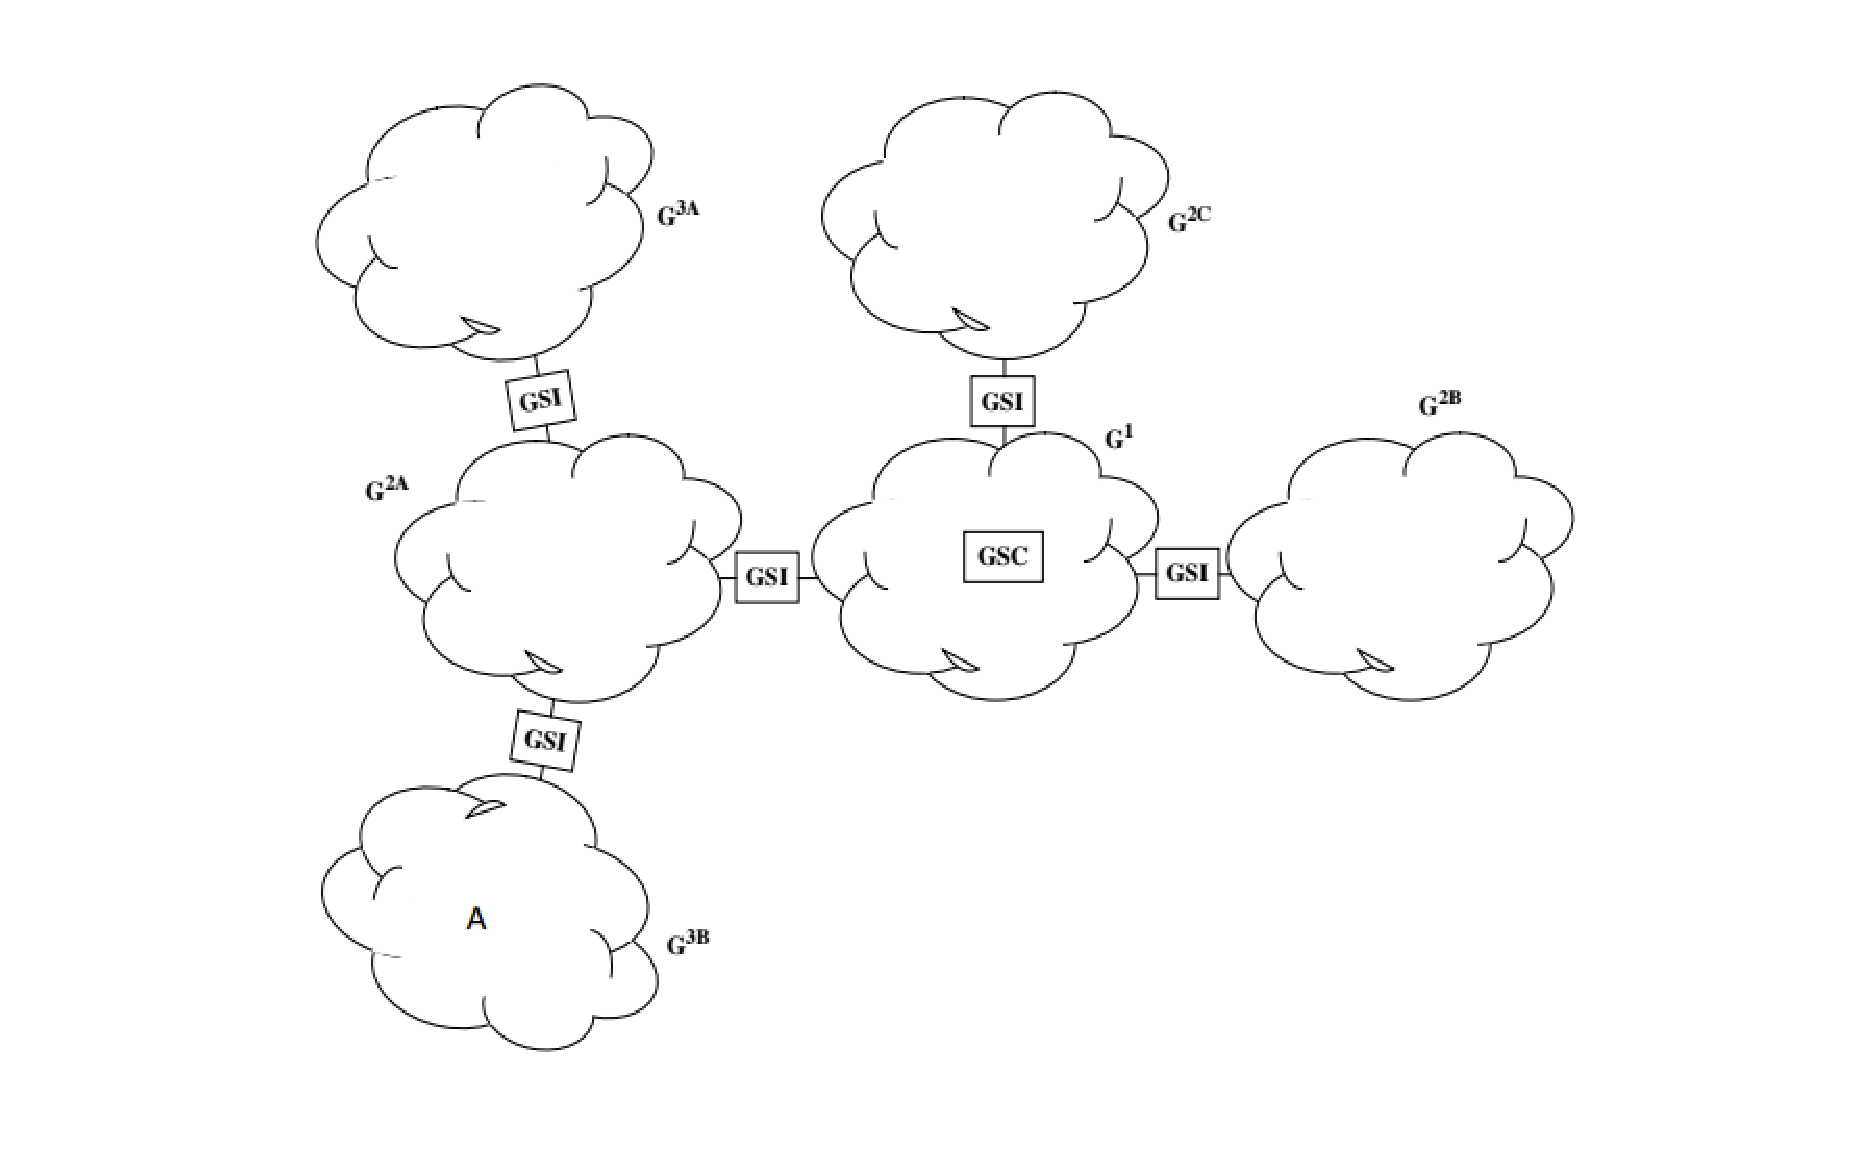
\includegraphics[scale=0.5]{one.eps}
\end{center}
\noindent\textbf{Assume the GSC is distributing a new group key to the to the group members using Iolus. How many times will this new key be encrypted and decrypted before A learns the value of the new key? Also describe what entity performs each of the encryptions and decryptions.} \\
The new key will be first encrypted by the $GSC$ and sent to the $GSI$ of the $G^{2A}$. The $GSI$ of $G^{2A}$ will decrypt the new key, then re-encrypt the key for the $GSI$ of subgroup $G^{3B}$. Once the $GSI$ of $G^{3B}$ recives the encrypted key the $GSI$ will decrypt it and once again encrypt for the user $A$. The last step will be user $A$ reciving \\
\textbf{Encryptions:} 3 \\
\textbf{Decryptions:} 3 \\


\section{[12] Key Trees}
\begin{center}
    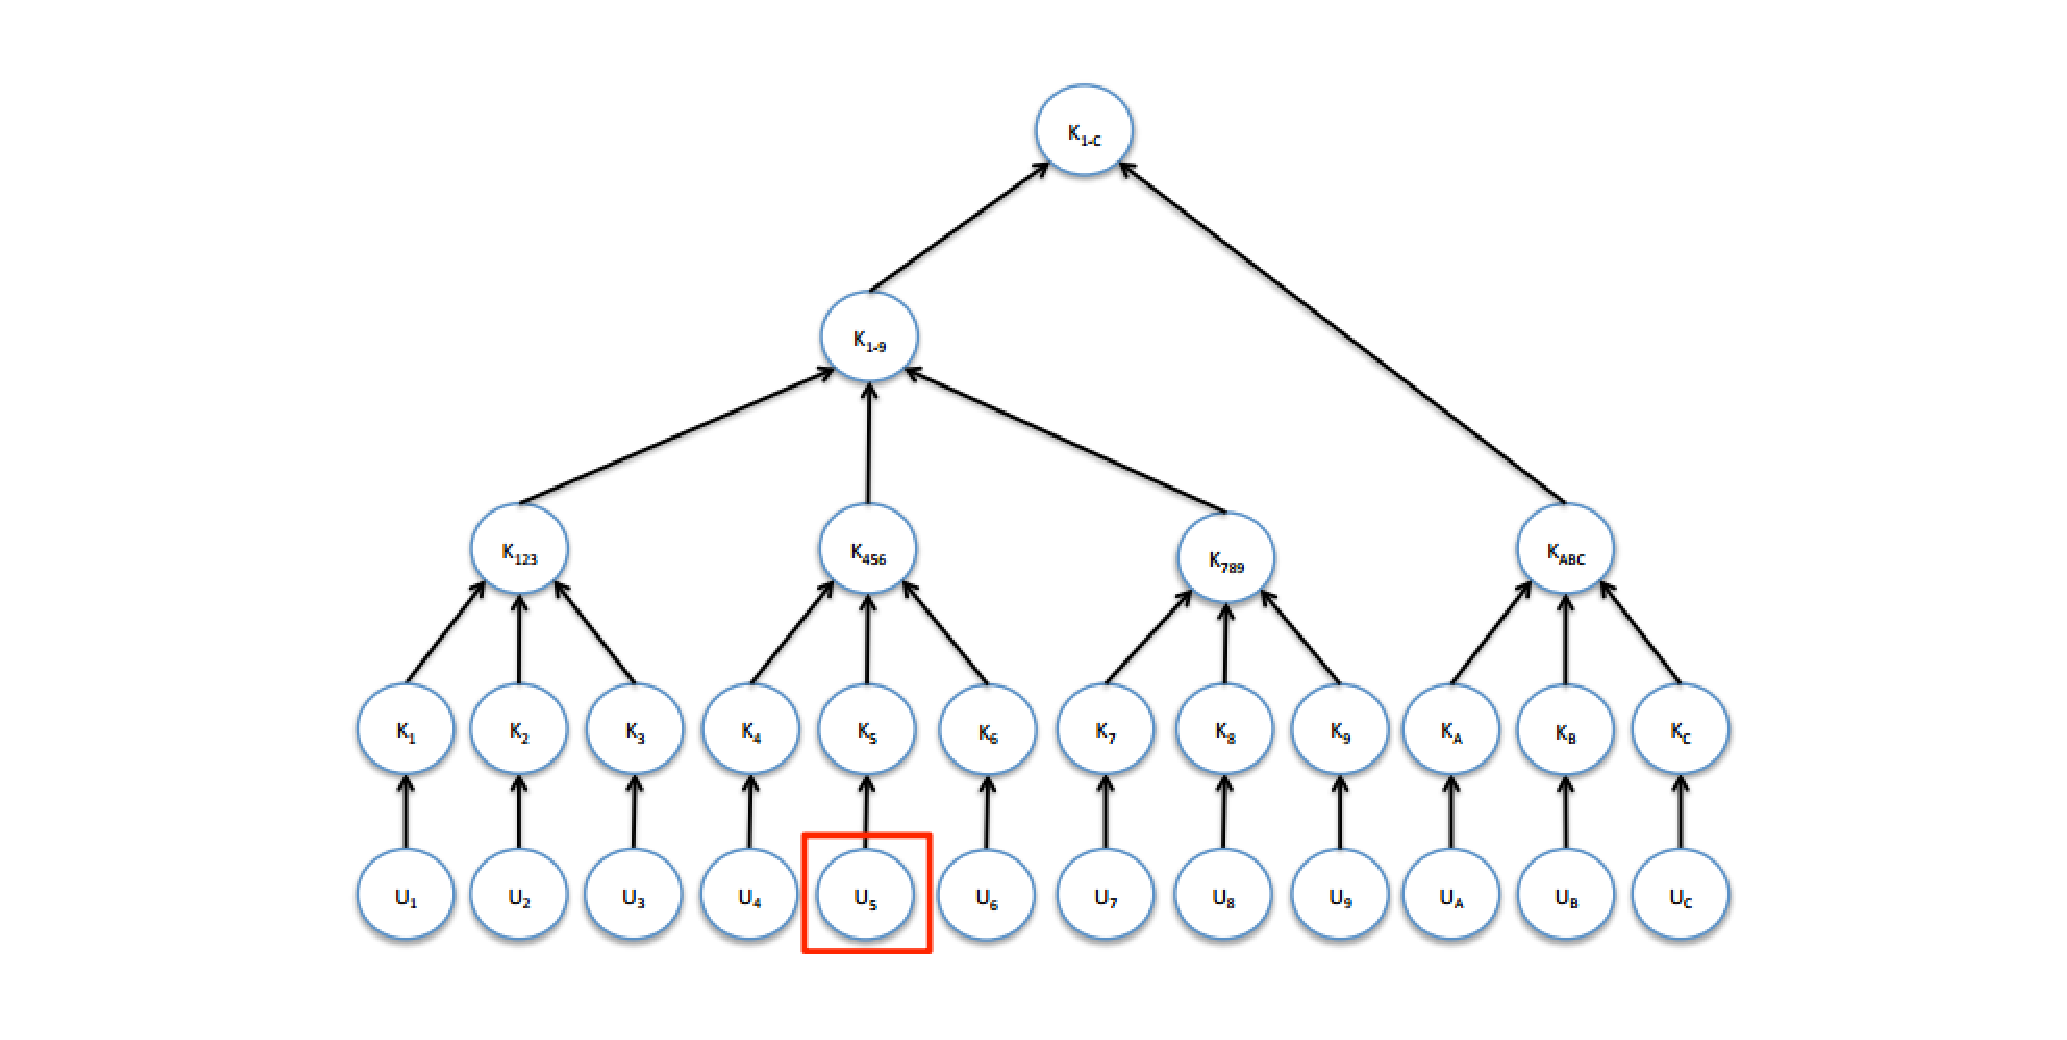
\includegraphics[scale=0.5]{three.eps}
\end{center}

\noindent\textbf{(6 points) If u5 is removed from the group, what keys should be changed? Write down how keys are distributed with each required step. Assume user oriented re-keying.} \\
If the $u_{5}$ is removed from the key tree, then $k_{1-c}$, $k_{1-9}$, and $k_{456}$ should change. \\

\begin{tabular}{l c l}
    $s \rightarrow \{u_{1},\dots,u_{c}\}$ & : & $\{k_{1-9}\}_{k_{1-c}}$ \\
    $s \rightarrow \{u_{4},u_{6}\}$ & : & $\{k_{1-9}, k_{4-6}\}_{4,6}$ \\
    $s \rightarrow u_{5}$ & : & $\{k_{1-9},k_{4-6}\}_{k5}$ \\
\end{tabular}


\noindent\textbf{(6 points) Assume a new member is added (at now vacant location u5 ). Write down how keys are distributed with each required step. Assume key-oriented re-keying.} \\

\begin{tabular}{l c l}
    $s \rightarrow \{u_{1},\dots,u_{c}\}$ & : & $\{k_{1-9}\}_{k_{1-c}}$ \\
    $s \rightarrow \{u_{4},u_{6}\}$ & : & $\{k_{1-9}, k_{4-6}\}_{4,6}$ \\
    $s \rightarrow u_{5}$ & : & $\{k_{1-9},k_{4-6}\}_{k5}$ \\
\end{tabular}

\section{[20] SSL/TSL}
\noindent\textbf{(10 points) What is ``The Heartbleed Bug'', describe in detail how it works against SSL, and how it can be present.} \\
The ``Heartbleed Bug'' was a serious weakness in the OpenSSL library. The bug allows specially crafted packet that triggers a use after free attack. In the vulnerable version of OpenSSL the size of the message is sent with the message itself and is never verified. An adversary can exploit this bug by sending a very small message but say it is much larger. This will make the server allocate more memory than is needed for the message. The memory that is allocated ``could'' contain sensitive data including
X.509 certificate secret keys, usernames, passwords, or other data. The sensitive data would be returned to the adversary upon request for their message. 

\noindent\textbf{(10 points) The proper key exchange and cipher suite choices for SSL/TLS continually change. We have discussed a potential key exchange mode and cipher suite selection that would be a reasonable choice at this moment during the class (also with an email). Write down some of the algorithms (discussed on the board), and also state what should be an ultimate care while you configure SSL/TLS (especially while doing international business).} \\



\section{[14] Needham-Schroeder, Otway-Rees}
\noindent\textbf{(12 points) In the Needham-Schroeder protocol (extended version in slides)}
\begin{enumerate}[label=\roman*]
    \item\textbf{(2 points) How is Alice authenticated by the KDC?} \\
        The KDC will send an encrypted message with Alice's public key. Alice should be the only one to decrypt this message as she is the only one with her secret key. 
    \item\textbf{(2 points) How is Bob authenticated by the KDC?} \\
        Bob will send an encrypted nonce to Alice encrypted by Bob's secret key. Alice will send this encrypted nonce to the KDC in message \#3 which if Bob is authentic the KDC will be able to decrypt the nonce. 
    \item\textbf{(2 points) How is the KDC authenticated to Alice?} \\
        Alice is authenticated to the KDC through the trust of Bob. After the KDC sends Alice the ``Ticket to Bob'' and Alice forwards that to Bob, if Bob responds then then Alice can authenticate the KDC.
    \item\textbf{(2 points) How is the KDC authenticated to Bob?} \\
        The KDC is authenticated to Bob through the nonce that was sent to Alice and put in the ''Ticket to Bob''.
    \item\textbf{(2 points) How Alice is authenticated to Bob?} \\
    \item\textbf{(2 points) How Bob is authenticated to Alice?}
        Because both Alice and Bob trust the KDC the generated shared key $K_{ab}$ will be authenticate mutually between Alice and Bob.
\end{enumerate}

\noindent\textbf{(2 points) In the Needham-Schroeder protocol, Alice is the party that is in contact with the KDC, but in the Otway-Rees protocol, Bob is the party that is in contact with the KDC. Explain why this is the case.} \\
This reduces the work load that the KDC will need to process. Bob will be able to determine if Alice is not legitimate quicker since he is the one talking to the KDC.

\section{[14] Kerberos}
\noindent\textbf{(3 points) When Bob receives a ticket from Alice, how does he know it is genuine?} \\
Bob will directly send the encrypted token to the KDC in the second message. If the KDC verifies that Alice is authentic then comunication will continue, if not then Bob knows that Alice is a fraud.

\noindent\textbf{(3 points) When Bob receives a ticket from Alice, how does he know it came from Alice?} \\
In the second message when Bob is authenticating Alice in message 2, the message to the KDC contains both of their Names and tokens encrypted under their private keys. If the name of Alice and her encrypted message do not pass verification from the KDC then Bob will know it did not come from Alice.

\noindent\textbf{(3 points) When Alice receives a replay, how does he know it came from Bob (that it is not a replay of an earlier message from Bob)?} \\
\begin{center}
    ** I am assuming ''replay'' in this question is a typo and should have been \textit{reply}. **
\end{center}
Alice will know that the message is from Bob since the message contains the nonce set in the first message directly to Bob, that was encrypted under her private key. 

\noindent\textbf{(5 points) What does the Ticket contain that allows Alice and Bob to communicate securely?} \\
The ticket contains a shared key that is unique to only Alice and Bob. Because the KDC, Bob, and Alice have all been authenticated, further comunication between Alice and Bob are secure. However, if the KDC is compramized then all security is void.

\medskip
\bibliography{quinnsaHW3}
\bibliographystyle{ieeetr}
\end{document}
